\subsubsection{Impact of Different Types of Program Graphs}
\label{sec:graphs}

\begin{figure}[thbp]
\begin{center}
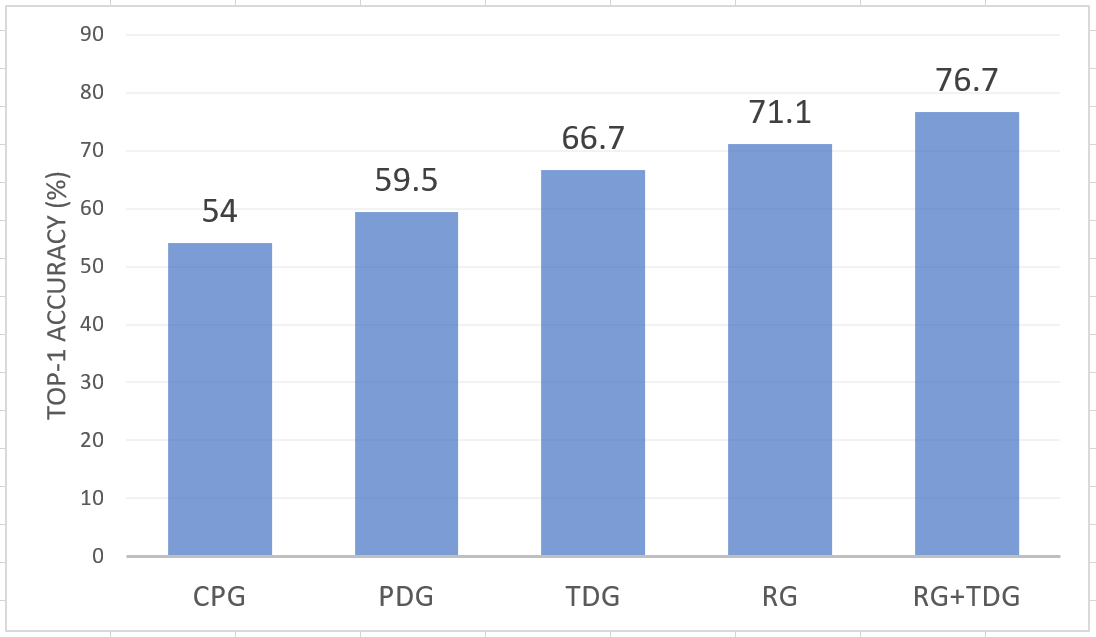
\includegraphics[width=2.8in]{figures/sensi-graphs-name}
\vspace{-8pt}
\caption{RQ3. Impact of Input Graph on Variable Name Prediction}
\label{graph-name-result}
{\bf CPG}: Code Property Graph, {\bf PDG}:Program Dependence Graph, {\bf TDG}: Type Dependency Graph, {\bf RG}:Relation Graph. 
\end{center}
\end{figure}

\begin{figure}[thbp]
\begin{center}
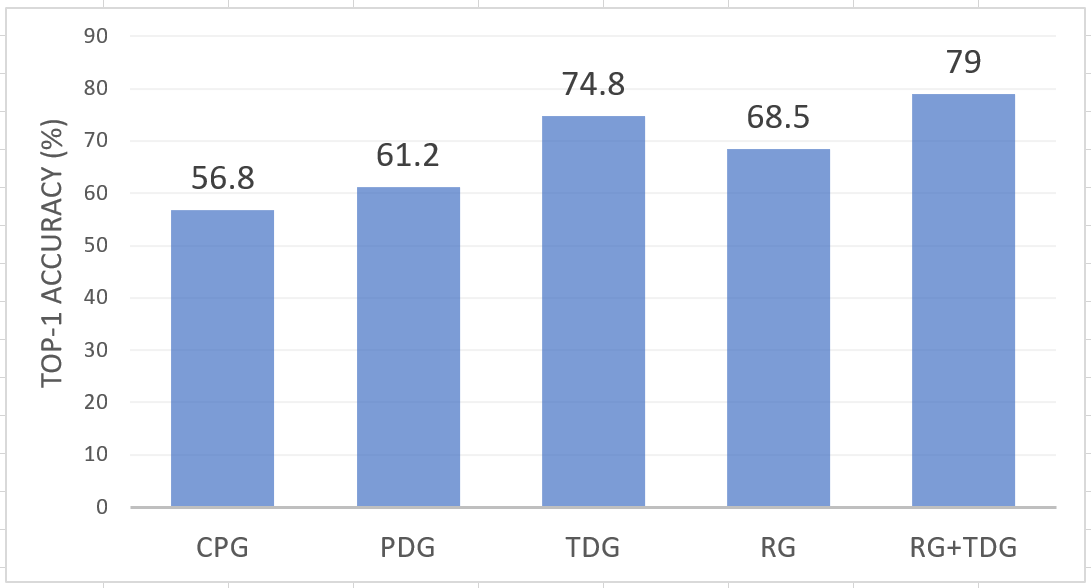
\includegraphics[width=2.8in]{figures/sensi-graphs-type}
\vspace{-8pt}
\caption{RQ3. Impact of Input Graph on Variable Type Prediction}
\label{graph-type-result}
{\bf CPG}: Code Property Graph, {\bf PDG}:Program Dependence Graph, {\bf TDG}: Type Dependency Graph, {\bf RG}:Relation Graph.
\end{center}
\end{figure}

As in any approach, the representation for source code is important
and affects the final performance. In this experiment, we kept the
same neural network architecture, however, changed different input
graphs extracted from source code. In addition to the graphs used in
{\tool} (relation graph (RG), type dependency graph (TDG)), we also
experimented with program dependence graph (PDG) and code property
graph (CPG)~\cite{tien} because they are popularly used in several
machine learning approaches for source code.
